\subsection{Leptonically decaying boson}
\label{subsec:leptons_selection}

Events are categorized into 0-, 1- and 2-lepton channels by number of Loose leptons in the final state. The common definition of Loose lepton (see Sec.~\ref{sec:ObjectDefinition}) ensures three channels to be orthogonal. 
Basically we can follow the event selections used in the previous analysis based on the 36\,\ifb dataset\cite{Ryzhov:2310214}.
This section focuses on the dedicated selection we have for the three leptons channels.

%%% 0-lepton channel
\subsubsection{0-lepton channel}
\label{subsubsec:0lep_event_selection}

The 0-lepton channel requires events containing a $\nu\nu$ pair from a $Z$ boson decay and boosted $W/Z \to q\bar{q}$ candidate defined in Section~\ref{subsubsec:merged_jets_selection}. 
The $Z \rightarrow \nu\nu$ identification requires no Loose lepton and high missing energy in the final state.

Several anti-QCD cuts are applied to reject the QCD multijet and non-collision background. 
\begin{itemize}
\item $\met >$ 200 GeV,
\item $\mpt >$ 50 GeV,
\item $\Delta\phi(\met,\mpt) < \pi/2$
\item $\min(\Delta\phi(\met,j)) > \pi/6$ and 
\item $\Delta\phi(\met, Sig-J) > \pi/9$ (merged regime)
\item $\Delta\phi(\met, Sig-jj) > \pi/9$ (resolved regime)
\end{itemize}

where 
$\mpt$ is the track-based missing momentum, 
$\min(\Delta\phi(\met,j))$ is the minimum azimuthal difference between \met and small-R jets, 
$\Delta\phi(\met, \mpt)$ is the azimuthal difference between \met and \mpt,
and $Sig-J$/$Sig-jj$ are the signal jets candidate in the merged/resolved regime. 

Merged and resolved regime selections are discussed in details in Section \ref{subsec:sr_selection}.

The QCD multijets background are highly suppressed by these selections, as shown in Figure~\ref{fig:0lepAntiQCD}. 
\begin{figure}[ht]
	\centering
		\subfigure[$E_\text{T}^\text{miss,track} > 50~\text{GeV}$]{\includegraphics[width=0.3\textwidth]{figures/0lep/cutflow/nominal/merged/plots/individual_SRVBS_HP_TrkMET_TrkMET_cutflow.pdf}}
    	\subfigure[$|\Delta\Phi(E_\text{T}^\text{miss},E_\text{T}^\text{miss,track})|/\pi<\frac{1}{2}$]{\includegraphics[width=0.3\textwidth]{figures/0lep/cutflow/nominal/merged/plots/individual_SRVBS_HP_DPhiMETTrkMET_DeltaPhiMetTrkMet_cutflow.pdf}}
    	\subfigure[$\text{min}\{|\Delta\Phi(E_\text{T}^\text{miss},j^\text{smallR}_i)|\}_i/\pi > \frac{1}{6}$]{\includegraphics[width=0.3\textwidth]{figures/0lep/cutflow/nominal/merged/plots/individual_SRVBS_HP_MinDPhiSmallRJets_MinDPhiSmallRJets_cutflow.pdf}}\\
    	\subfigure[$|\Delta\Phi(E_\text{T}^\text{miss},J^\text{sig})|/\pi > \frac{1}{9}$]{\includegraphics[width=0.3\textwidth]{figures/0lep/cutflow/nominal/merged/plots/individual_SRVBS_HP_MinDPhiFatJet_MinDPhiFatJet_cutflow.pdf}}
    	\subfigure[$|\Delta\Phi(E_\text{T}^\text{miss},(jj)^\text{sig})|/\pi > \frac{1}{9}$]{\includegraphics[width=0.3\textwidth]{figures/0lep/cutflow/nominal/merged/plots/individual_SRVBS_Res_MinDPhiDijet_MinDPhiDijet_cutflow.pdf}}
        \caption{Anti-QCD selection cuts in the 0-lepton channel. Shown are all events passing the event selection (see Tab. \ref{tab:0lepCutFlow}) up to the cut that is shown. The cuts common for both merged and resolved regimes (a-c) are shown for the merged SR HP selection (Tab. \ref{tab:0lepCutFlow} a) while the cuts that only apply for one of the regimes (d: merged, e: resolved) are shown for the merged SR HP (Tab. \ref{tab:0lepCutFlow} a) or resolved SR (Tab. \ref{tab:0lepCutFlow} c) respectively. 
%\textcolor{red}{(binning has to be updated, consistent symbols for MET [Tobias])}
Note: 'stop' is referring to SM single-top process.
} 
    \label{fig:0lepAntiQCD}
\end{figure}

The observed data not described by the simulated events are coming from multijet and non-collision background.
These backgrounds are primarily a result of a mis-measurement of a single jet's energy resulting in a direction of $\met$ aligned to the direction of that jet and an amplitude of $\met$ large enough to pass the $\met$ trigger and preselection cuts applied in the 0-lepton channel.
The definition of $\mpt$ does not involve jets but relies on the information of the inner tracker while the calculation of $\met$ also includes information on jets.
As a result multijet and non-collision background tends to have a smaller amplitude in $\mpt$ and large difference in the direction of $\mpt$ and $\met$.
The background rejection is achieved by the cut on $\mpt$ and $\Delta \phi(\mpt,\met)$, and $\min \Delta \phi(\met, j)$ (Figure~\ref{fig:0lepAntiQCD} a--c).
After subsequent cuts on the distance between \met and the signal jets (Figure~\ref{fig:0lepAntiQCD} d--e), the fraction of the remaining multijet events is negligibly small with respect to the other uncertainties.


%%% 1-lepton channel
\clearpage
\subsubsection{1-lepton channel}
\label{subsubsec:1lep_event_selection}
This section summarizes the SR definitions in 1-lepton channel.

\textbf{$W \to \ell\nu$}

To select events consistent with $W \to \ell\nu$ candidate, exactly one Tight lepton is required. In addition,
the following cuts are defined for all regions as common cuts:

\begin{itemize}
\item $\met > 80 \,\GeV$
\item $\ptl > 28 \,\GeV$ %and \textcolor{red}{I think this is related to lepSF binning} 
%\item $m_{J} > 50 \, \GeV$ (merged only)
\end{itemize}
are applied in the merged (resolved) analysis to suppress the multi-jet background.
Merged and resolved regime selections are discussed in details in Section \ref{subsec:sr_selection}.

Examples of distributions for MC samples as well as observed data are shown in Figure \ref{fig:1LepPreselCuts}; in particular, we can nicely see the W-peak in the $t\bar{t}$ process.

%\textcolor{red}{do we have any d-phi selection in 1-lep?? NO , this comment can be deleted after}

\begin{figure}[ht]
\centering
	\subfigure[$E_{T,miss}$ before any event selection.]{\includegraphics[width=0.3\textwidth]{figures/1lep/CRPlots/C_0ptag0pjet_0ptv_ALL_MET_Lin.png}} 
	\subfigure[$E_{T,miss}$ after merged common preselection.]{\includegraphics[width=0.3\textwidth]{figures/1lep/CRPlots/C_0ptag0pjet_0ptv_Presel_Merged_MET_Lin.png}} 
	\subfigure[$E_{T,miss}$ distribution after resolved common preselection.]{\includegraphics[width=0.3\textwidth]{figures/1lep/CRPlots/C_0ptag0pjet_0ptv_Presel_Resolved_MET_Lin.png}} \\

	\subfigure[$p_{T,l}$ before any event selection.]{\includegraphics[width=0.3\textwidth]{figures/1lep/CRPlots/C_0ptag0pjet_0ptv_ALL_PtL_Lin.png}} 
	\subfigure[$p_{T,l}$ after merged common preselection.]{\includegraphics[width=0.3\textwidth]{figures/1lep/CRPlots/C_0ptag0pjet_0ptv_Presel_Merged_PtL_Lin.png}} 
	\subfigure[$p_{T,l}$ distribution after common resolved preselection.]{\includegraphics[width=0.3\textwidth]{figures/1lep/CRPlots/C_0ptag0pjet_0ptv_Presel_Resolved_PtL_Lin.png}} \\

	\subfigure[$M_{J}$ before any event selection.]{\includegraphics[width=0.3\textwidth]{figures/1lep/CRPlots/C_0ptag0pjet_0ptv_ALL_MFatJet_Lin.png}} 
	\subfigure[$M_{J}$ after merged common preselection.]{\includegraphics[width=0.3\textwidth]{figures/1lep/CRPlots/C_0ptag0pjet_0ptv_Presel_Merged_MFatJet_Lin.png}} 

	\caption{Distributions for $E_{T,miss}$, $E_{T,miss}$, and $m_{J}$ in the 1 lepton channel at different stages of the analysis selection; preselection merged and preslection resolved labels refers to the set of cuts applied in the merged and resolved regime rather than the boson tagger cuts (merged) and the signal jets mass window cut.}
	\label{fig:1LepPreselCuts}
\end{figure}
%After the $W \to \ell\nu$ selection above and $W/Z \to jj$ selection described in Section~\ref{subsubsec:resolved_jets_selection},
%the following selection cuts are required to take the event topology of which two high-\pt\ bosons are back--to--back in the $x$--$y$ plane:
%\begin{itemize}
%\item $\Delta \phi(\ell, \met)< XX$;
%\item $\Delta \phi(j1,j2) < XX$;
%\item $\Delta \phi(\ell,j1(2)) > XX$;
%\item $\Delta \phi(j1(2), \met) > XX$;
%\end{itemize}
%where $\Delta \phi(i, j)$ is the distance in the  coordinate between objects $i$ and $j$.

%%% 2-leptons channel
\clearpage
\subsubsection{2-lepton channel}
\label{subsubsec:2lep_event_selection}

\textbf{$Z \to \ell\ell$}

The $Z \rightarrow \ell\ell$ candidates are identified by requiring two isolated same-flavour leptons (electrons or muons) satisfying Loose criteria defined in Section~\ref{subsec:electron_selection}--\ref{subsec:muon_selection}.
Both the leading and sub-leading lepton \pt are required to be $\pt > 27\,\GeV$, while it was $>28\,\GeV$ and $20\,\GeV$ in the previous analysis. 
%\textcolor{red}{do we have some optimisation study?}

Opposite charges are required for the muon pairs but not for the electron pairs. Electrons are more susceptible to charge mis-identification due to the conversions of photons from bremsstrahlung, especially at high \et. 
The dilepton invariant mass $m_{\ell\ell}$ is required to be consistent with the $Z$ boson mass. For electrons, a fixed $m_{\ell\ell}$ window:
\begin{equation}
83 < m_{ee} <  99\,\GeV
\end{equation}
is applied.
To account for the effect of dimuon mass-resolution degradation at high transverse momentum (\ptll), a \ptll-dependent mass window:
\begin{equation}
\left(85.6 - 0.0117\ptll\right) < m_{\mu\mu} <  \left(94.0 + 0.0185\ptll\right)\,\GeV
\end{equation}
is used for muons, which was optimized from the 2015+16 analysis~\cite{EXOT-2016-29}. 
For both electrons and muons, the mass windows are chosen to ensure that the $Z \to \ell\ell$ selection efficiency is approximately 95\% and independent of the heavy resonance mass. 
Events with additional leptons passing the Loose criteria are vetoed.

Data and MC distributions of relevant lepton distributions at the early stage 
of the selection are shown in Figure \ref{fig:2lepLeptons}; 
in particular, leptons \pt are shown after the lepton pre-selection 
while the dilepton invariant mass distribution is shown with those cut not applied.
The nice and clear $Z \rightarrow ll$ peak is visible in data in the $ll$ invariant mass distribution.

%In particular, modelling of the leading and sub-leading muon \pt look slighlty different. 
%This is an effect of the first bin in both distributions that has different values in the 
%data/MC ratio. After removing the first bin in the subleading muon \pt distribution the modelling
%qfor the two muons \pt is consistent as checked in Appendix \ref{app:leptonin2lep}.

\begin{figure}[ht]
	\centering
	\subfigure[Leading electron \pt]{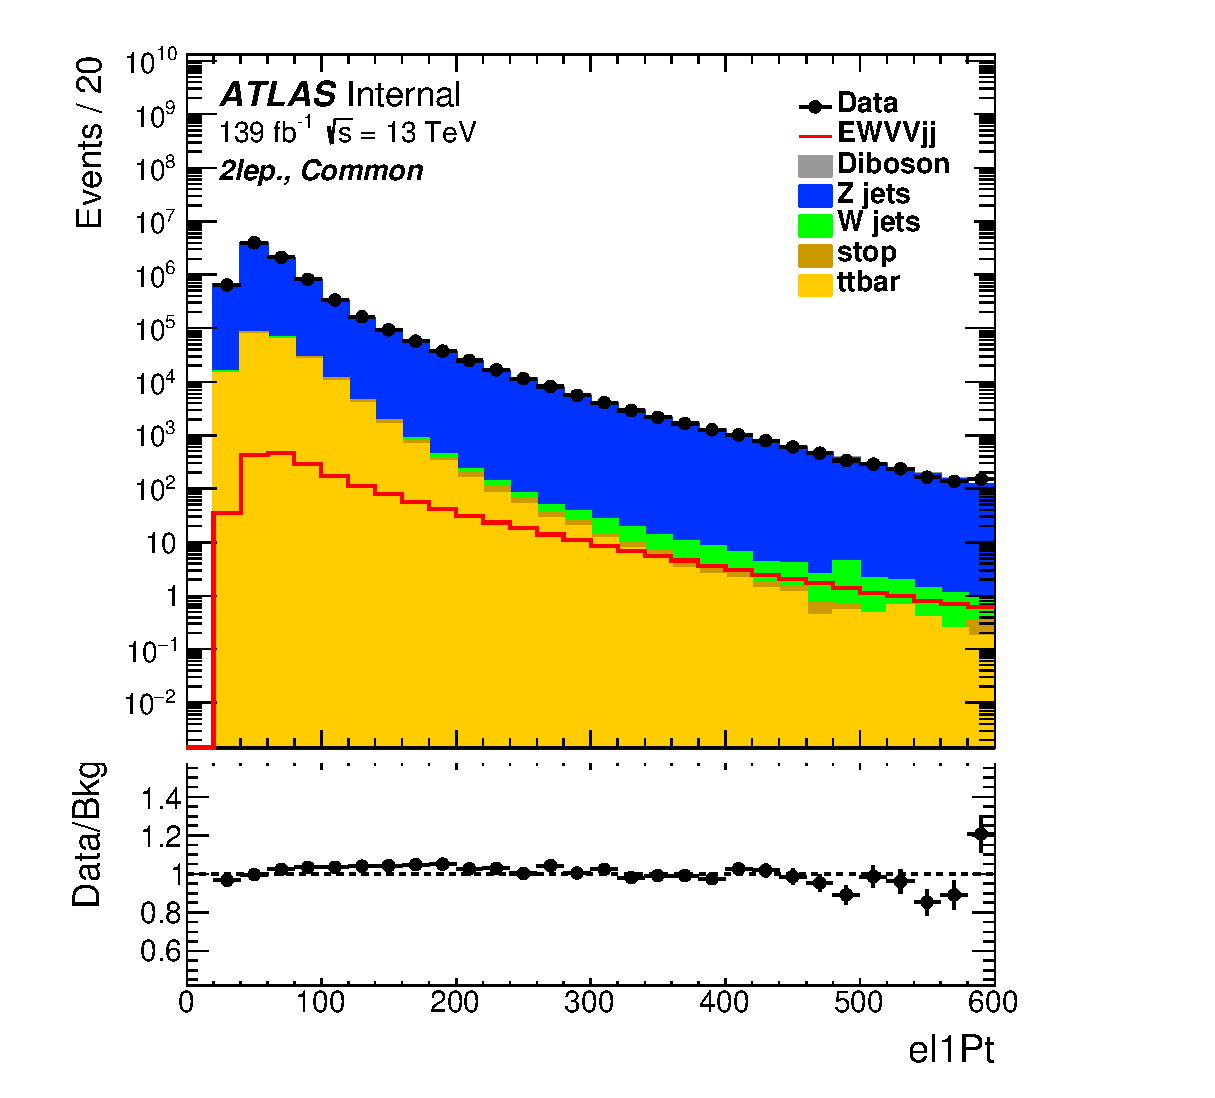
\includegraphics[width=0.3\textwidth]{figures/2lep/dataMC/C_0ptag1pfat0pjet_0ptv_Common_el1Pt_Log.eps}}
	\subfigure[Subleading electron \pt]{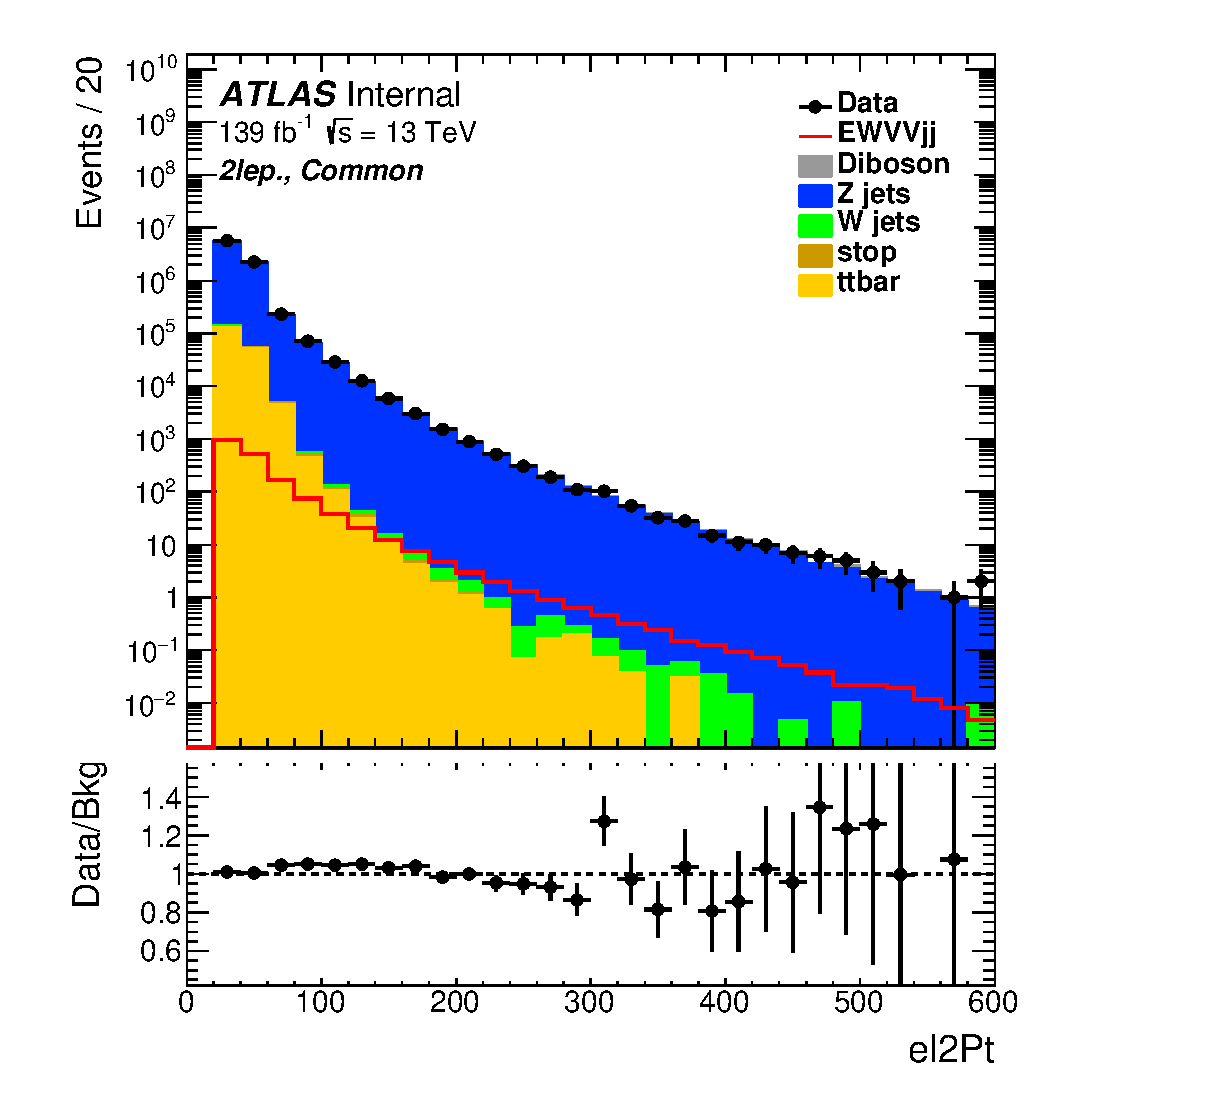
\includegraphics[width=0.3\textwidth]{figures/2lep/dataMC/C_0ptag1pfat0pjet_0ptv_Common_el2Pt_Log.eps}} \\
	\subfigure[Leading muon \pt]{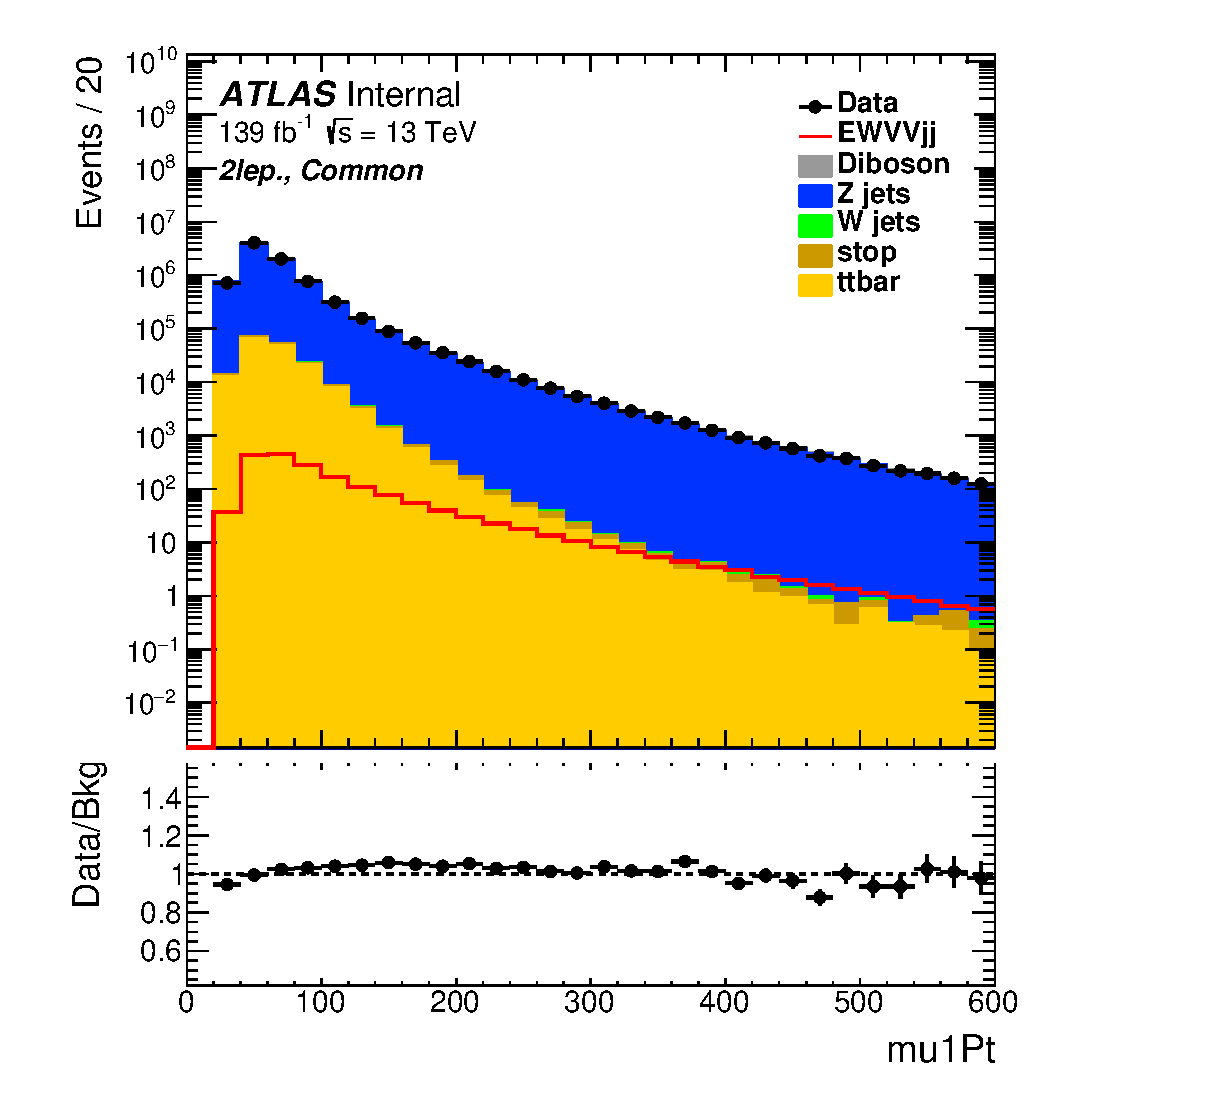
\includegraphics[width=0.3\textwidth]{figures/2lep/dataMC/C_0ptag1pfat0pjet_0ptv_Common_mu1Pt_Log.eps}}
	\subfigure[Subleading muon \pt]{\includegraphics[width=0.3\textwidth]{figures/2lep/dataMC/C_0ptag1pfat0pjet_0ptv_Common_mu2Pt_Log.eps}} \\
	\subfigure[\mll]{\includegraphics[width=0.3\textwidth]{figures/2lep/dataMC/C_0ptag1pfat0pjet_0ptv_ALL_llMass_Lin.png}}
	\caption{Lepton distributions in 2-lepton channel just after $M_{ll}$ window selection. The events before any selections are shown for Z mass peak,which is $M_{ll}$ distribution in plot (e).}
    \label{fig:2lepLeptons}
\end{figure}

